\documentclass[a4paper,12pt]{article}

\usepackage[utf8]{inputenc}
\usepackage{amsmath, amssymb}
\usepackage{graphicx}
\usepackage{geometry}
\usepackage{hyperref}
\usepackage{setspace}
\usepackage{fancyhdr}
\usepackage{float}
\usepackage{lipsum}
\usepackage{listings}
\usepackage{xcolor}
\usepackage{xcolor-material}

\geometry{margin=1in}

\pagestyle{fancy}
\fancyhf{}
\fancyhead[L]{Laporan Final Sistem Tertanam}
\fancyhead[R]{\thepage}

\lstdefinestyle{mystyle}{
    backgroundcolor=\color{white},
    commentstyle=\color{green},
    keywordstyle=\color{magenta},
    numberstyle=\tiny\color{gray},
    stringstyle=\color{purple},
    basicstyle=\ttfamily\footnotesize,
    breakatwhitespace=false,
    breaklines=true,
    frame=single,
    captionpos=b,
    keepspaces=true,
    numbers=none,
    numbersep=10pt,
    showspaces=false,
    showstringspaces=false,
    showtabs=false,
    tabsize=2,
}

\lstset{style=mystyle}

\setlength{\parskip}{0.5em} % Adjust paragraph spacing
\setlength{\parindent}{0pt} % Remove paragraph indentation

\begin{document}
\begin{titlepage}
    \centering
    \vspace*{1cm}
    {\Large \textbf{Laporan Final \textit{Game PingPong} pada \textit{Dotmatrix Display}}}
    \vfill
    \vspace{2cm}

    
\includegraphics[width=0.4\textwidth]{./images/logo.png}
    \vfill

    \vspace{1cm}
    \begin{onehalfspace}
    \textbf{Dosen Pengampu}\\
    Eko Pramunanto, S.T. M.T.

    \vspace{1cm}

    \textbf{Disusun Oleh:}\\
    Muhammad Haekal Muhyidin Al-Araby\\
    5024221004\\
    Sistem Tertanam - A
    \end{onehalfspace}

    \vfill

    \textbf{DEPARTEMEN TEKNIK KOMPUTER\\
    FAKULTAS TEKNOLOGI ELEKTRO DAN INFORMATIKA CERDAS\\
    INSTITUT TEKNOLOGI SEPULUH NOPEMBER\\2024}
\end{titlepage}

\section{Gambaran Umum}
Pingpong atau tenis meja adalah salah satu olahraga yang dimainkan 2 orang yang saling berlawanan.
Untuk mendapat skor pemain harus memasukkan bola ke daerah lawan. Bola digerakkan dengan paddle. Pemain dapat
service, smash, maupun menangkis bola.

Project ini adalah implementasi dari pingpong ke dalam dotmatrix display dimana
player dapat mengendalikan paddle dengan slide potentiomenter dan smash dengan menekan button.
smash akan membuat bola bergerak lurus dan bertambah cepat.

Untuk memenangkan permainan Player harus mendapatkan skor lebih atau sama dengan 11 dan memiliki keunggulan 2 poin
dari lawan. Bila keunggulan tersebut tidak dimiliki maka permainan akan berlanjut terus menerus hingga keduanya mendapatkan skor 15
yang akan berakhir seri.

\section{Komponen}
\subsection{Normally Close Switch}
Saklar yang yang tertutup pada kondisi normal dan terbuka ketika ditekan. Dengan memanfaatkan pull-up internal
pada pin GPIO ESP32 dan menyambungkan ujung lainnya ke ground kita dapat mendapatkan nilai 1 ketika ditekan.
Pada project ini switch ini dimanfaatkan untuk player dapat melakukan smash saat ditekan.

\subsection{Slide Potentiometer}
Potentiometer jenis ini mengubah resistansi pada rangkaian dengan menggunakan mekanisme geser. Karena sifatnya
yang dapat menghasilkan data analog biasa digunakan untuk mengatur parameter suatu device dengan akurasi yang lebih
tinggi. Pada ESP32 kita dapat membaca nilai dari potentio meter ini dengan menggunakan pin ADC pada ESP32.
Pin ADC pada ESP32 dapat membaca nilai tegangan dengan rentang 0 - 3.3v setelah itu maka esp akan menunjukkan
nilai maksimum. Resolusi ADC dari ESP32 adalah dari rentang 0 - 12 dimana semakin tinggi resolusi akan semakin akurat namun
semakin berat juga pada performa. Pada project ini saya memilih 3 sebagai resolusi karena kita hanya membutuhkan
nilai 0 - 8. Karena hanya terdapat 8 pixel pada dotmatrix vertikal.

\subsection{Led DotMatrix 8x32}
Dotmatrix MAX7219 adalah modul untuk mengendalikan display dotmatrix 8x8 sebanyak 4 buah. Chip yang digunakan mampu
mengendalikan seluruh pixel pada dotmatrix. Informasi dikirimkan secara serial. Dan menyebar ke seluruh dotmatrix.
Led ini biasa digunakan untuk running text dan game interaktif.

\subsection{ESP32}

\section{Desain Sistem}
\subsection{Rangkaian Skematik}
\begin{figure}[H]
    \centering
    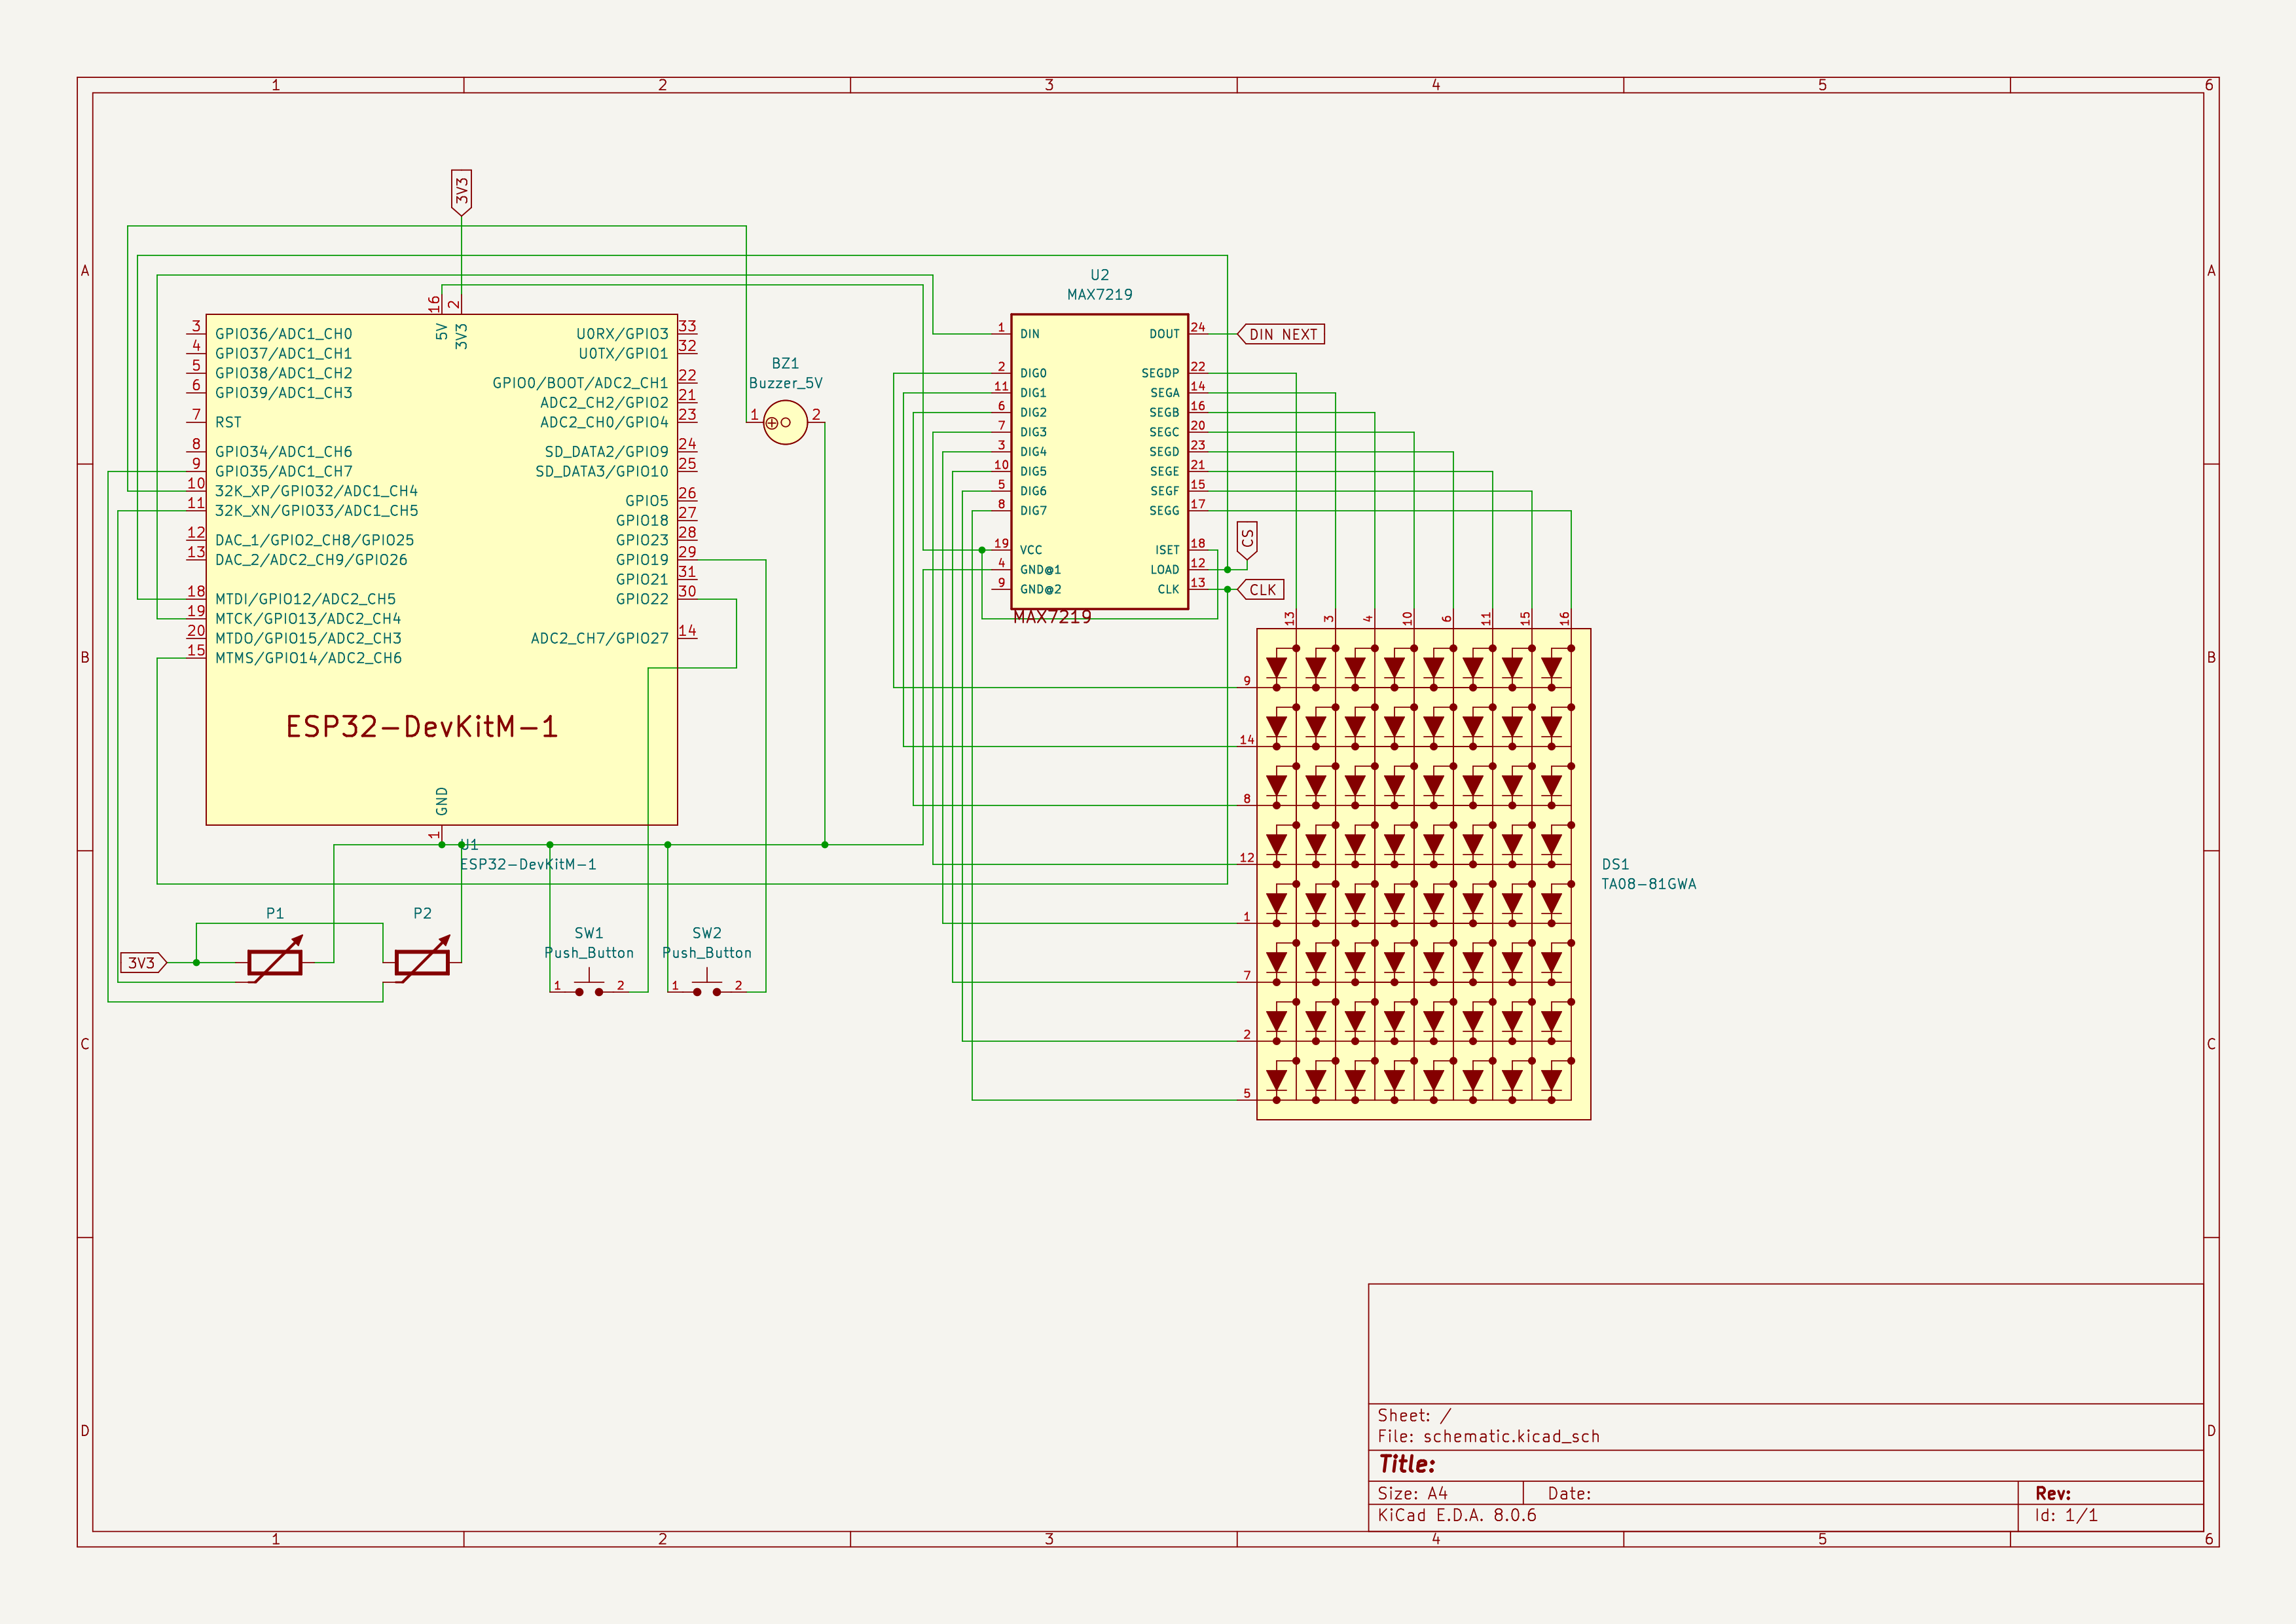
\includegraphics[width=1\textwidth]{images/schematic.png}
    \label{fig:schematic}
    \caption{Schematic}
\end{figure}
Rangkaian menggunakan ESP32 yang terhubung pada IC MAX7219 dimana CS
terhubung pada pin D12, DIN pada D13 dan clock pada D14
terdapat 4 IC MAX7219 yang saling terhubung secara seri. Lalu push button dihubungkan dengan
ground dan GPIO dan potentiometer dihubungkan ke ground, vcc, dan GPIO.
\subsection{Desain Game}
\begin{figure}[h!]
    \centering
    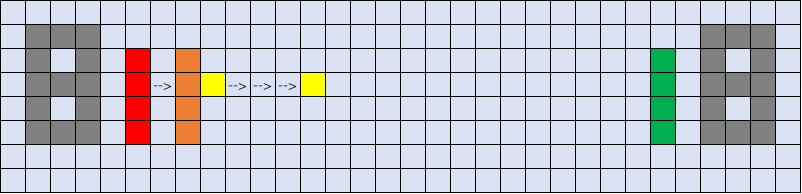
\includegraphics[width=1\textwidth]{images/desain_game.png}
    \label{fig:desaingame}
    \caption{Desain Game}
\end{figure}
\begin{enumerate}
    \item Game memiliki 2 player yang dapat digerakkan dengan slide potentiometer
    \item Bola akan memantul saat menabrak pembatas ataupun player
    \item Bola memantul secara diagonal dengan kecepatan konstan
    \item Bila player smash dan mengenai bola, bola akan bergerak lurus dan lebih cepat
    \item Bila bola melewati player maka player lainnya akan mendapatkan skor
    \item Player yang kebobolan akan mendapatkan bola dan dapat menggerakkannya
        dan menekan tombol smash untuk service.
    \item Game akan berakhir bila salah satu pemain mencapai skor 11 dan selisih 2 poin.
    \item Game akan berakhir imbang ketika kedua pemain mencapai 15 poin
\end{enumerate}

\subsection{Program}
\subsubsection{Menampilkan}
Untuk menampilkan ke dotmatrix dapat digunakan 2 library MD\_Parola dan MD\_MAX72xx. Dimana MD\_Parola dapat
menampilkan huruf namun kurang dalam kontrol sehingga akan kesulitan untuk menampilkan Game. Sehingga MD\_Parola hanya akan digunakan
saat menampilkan string. Sedangkan saat ingin menampilkan karakter akan menggunakan MD\_MAX72xx yang memberikan raw control pada
dotmatrix display. Untuk itu akan dibuat sebuah fungsi yang menerima input berbentuk array 8*32 untuk ditampilkan pada dotmatrix. Berikutnya
akan disebut frame. Lalu tiap objek akan diupdate dengan diletakan pada frame tersebut. Sesuai dengan posisi.

\subsubsection{Input}
Input didapatkan dengan mengambil nilai analogRead pada potentiometer dan digitalRead pada button smash.
\subsection{Source Code}
Berisi program utama yang mengatur main loop.
\lstinputlisting[language=C++, caption={main.cpp}]{../src/main.cpp}
Program di bawah mengendalikan device dotmatrix menggunakan library Parola dan MDMAX
\lstinputlisting[language=C++, caption={device.hpp}]{../include/device.hpp}
\lstinputlisting[language=C++, caption={device.cpp}]{../src/device.cpp}
Program di bawah menampilkan untuk menampilkan Intro
\lstinputlisting[language=C++, caption={animation.hpp}]{../include/animation.hpp}
\lstinputlisting[language=C++, caption={animation.cpp}]{../src/animation.cpp}
Program di bawah Berisi class vector2 untuk memudahkan posisi game object
\lstinputlisting[language=C++, caption={vector2.hpp}]{../include/vector2.hpp}
\lstinputlisting[language=C++, caption={vector2.cpp}]{../src/vector2.cpp}
Program di bawah berfungsi mendapatkan input player dan mengupdate state player
\lstinputlisting[language=C++, caption={player.hpp}]{../include/player.hpp}
\lstinputlisting[language=C++, caption={player.cpp}]{../src/player.cpp}
Program di bawah untuk mengupdate state bola
\lstinputlisting[language=C++, caption={ball.hpp}]{../include/ball.hpp}
\lstinputlisting[language=C++, caption={ball.cpp}]{../src/ball.cpp}
Program di bawah untuk menyalakan buzzer
\lstinputlisting[language=C++, caption={buzzer.hpp}]{../include/buzzer.hpp}
\lstinputlisting[language=C++, caption={buzzer.cpp}]{../src/buzzer.cpp}
Program di bawah untuk memunculkan skor
\lstinputlisting[language=C++, caption={score.hpp}]{../include/score.hpp}
\lstinputlisting[language=C++, caption={score.cpp}]{../src/score.cpp}
Program di bawah berisi Global Variabel yang digunakan seluruh program
\lstinputlisting[language=C++, caption={global.hpp}]{../include/global.hpp}
\lstinputlisting[language=C++, caption={global.cpp}]{../src/global.cpp}
\subsection{Hasil}
\begin{figure}[h!]
    \centering
    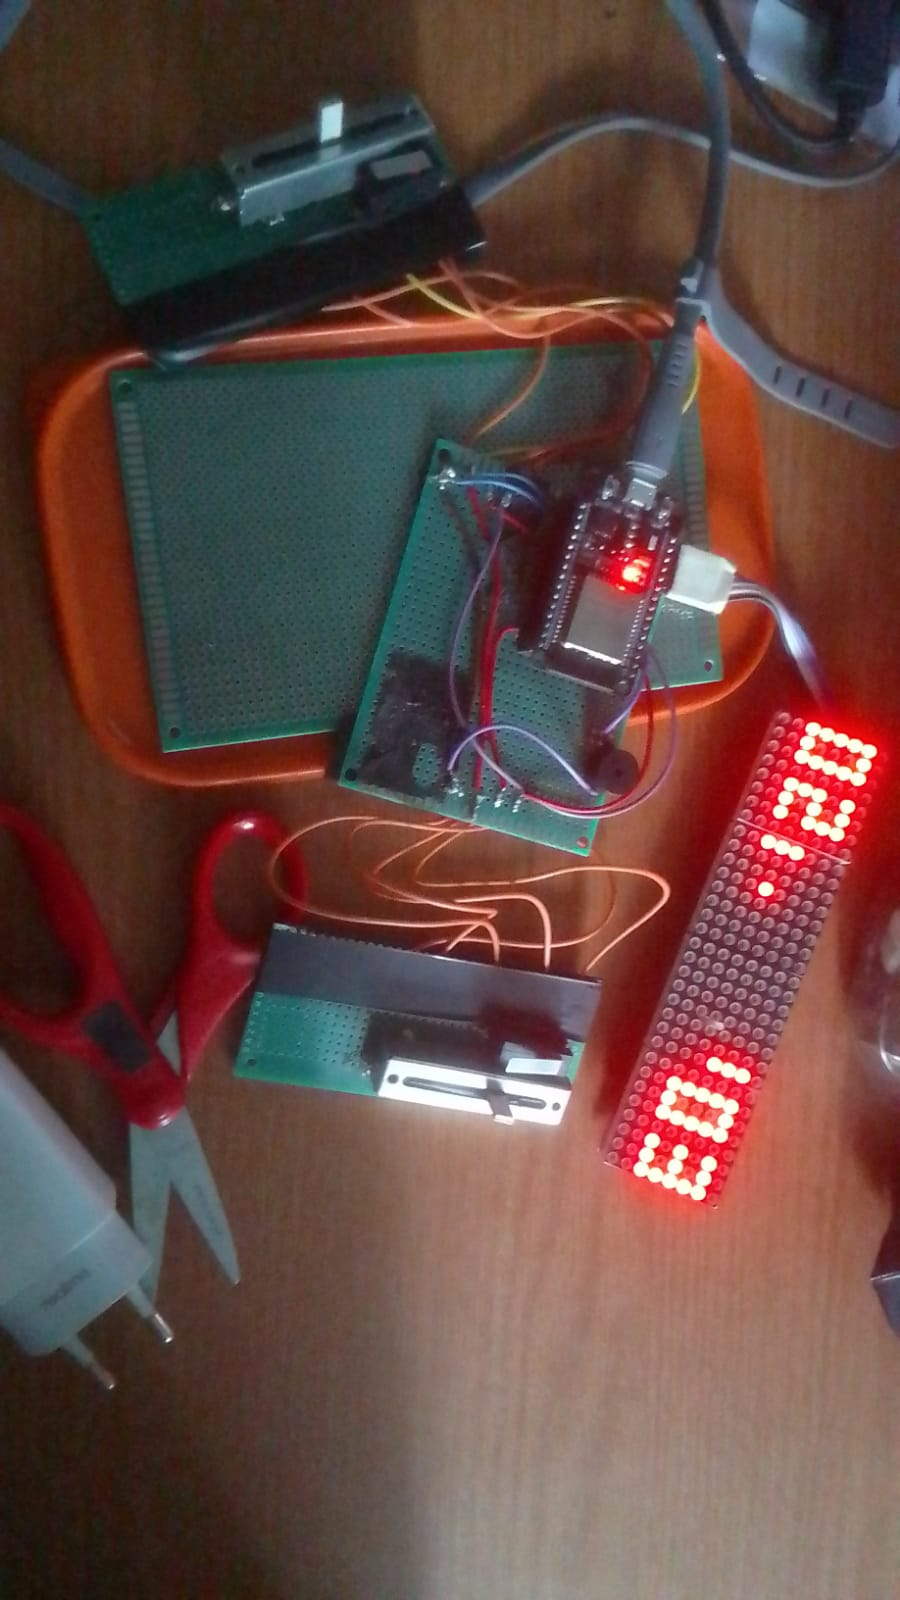
\includegraphics[width=0.5\textwidth]{./images/no-package.jpeg}
    \caption{Hasil tanpa package}
\end{figure}
\end{document}
